Come precedentemente specificato sono state estrapolate le entità principali intorno alle quali sviluppare la progettazione. Ciò è stato possibile grazie ad un'approfondita analisi del flusso aziendale, derivato direttamente dall'analisi delle azioni e dei processi interni.\newline
Il risultato è dato dalle quattro seguenti entità fondamentali: \newline

\noindent\makebox[\textwidth]{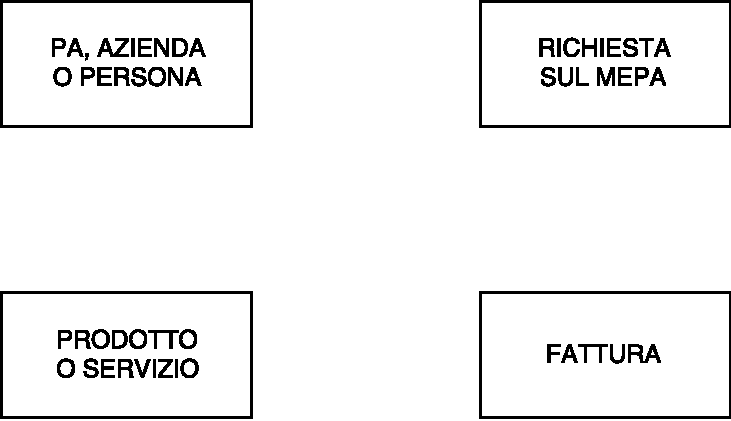
\includegraphics[width=\textwidth-5cm]{./immagini/entita_fondamentali.pdf}}
\newline
\newline
RICHIESTA SUL MEPA: il blocco rappresenta gli strumenti che le pubbliche amministrazioni utilizzano per  l'interfacciamento con la nostra azienda. In questo caso si parla di gare pubbliche oppure richieste di trattativa dirette. \newline
PA, AZIENDA O PERSONA: è il macrogruppo comprensivo delle entità giuridiche che hanno rapporti commerciali con la nostra azienda, tra questi ci sono i fornitori e i clienti, sia privati e pubbliche amministrazioni.\newline
PRODOTTO O SERVIZIO: comprende tutti i prodotti vendibili o acquistabili dall'azienda disponibili dai fornitori e i servizi disponibili.\newline
FATTURA: è l'entità fondamentale che interviene in tutte le operazioni sia per l'acquisto che per la vendita di prodotti e/o servizi.

\newpage
